По измеренным данным построим графики зависимости $h(t)$. По углу наклона прямой определим скорость движения уровня жидкости в капилляре.

% n = 0,3%

\begin{figure}[H]
	\centering
	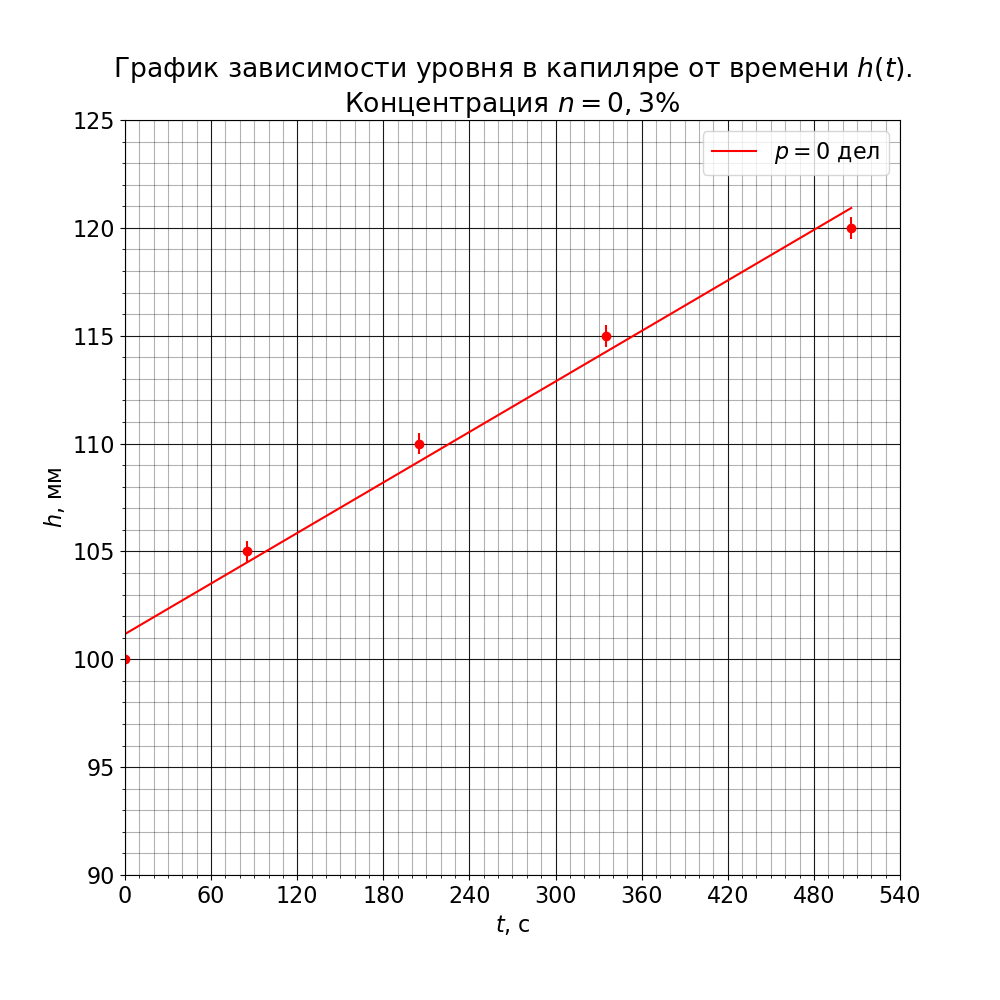
\includegraphics[width=1 \textwidth]{../plots/graph h_t n0.3 straight.png}
\end{figure}

С помощью метода наименьших квадратов проведём наилучшую прямую $h~=~vt~+~h_0$.

$P = 0$ дел. \\
$v = 0,039 \pm 0,003$ $\frac{мм}{с}$. \\
$h_0 = 101,2 \pm 0,8$ мм.

\begin{figure}[H]
	\centering
	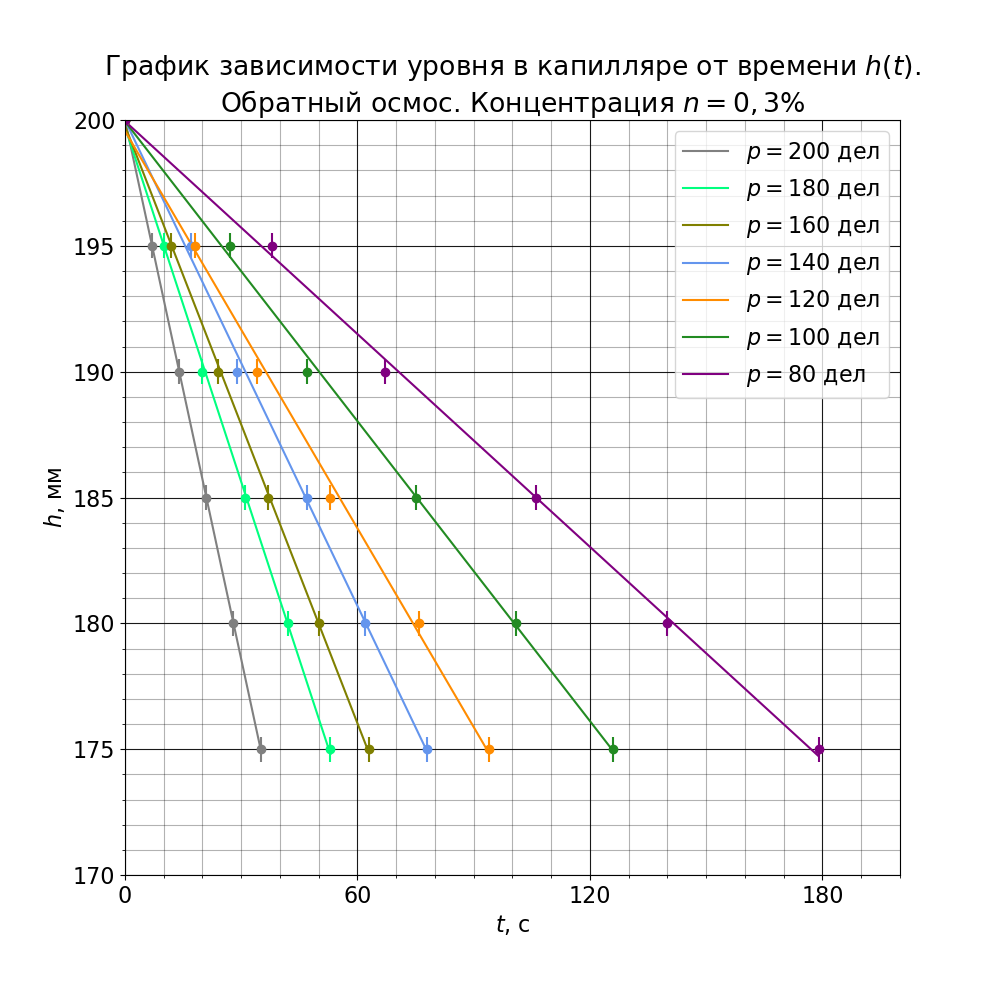
\includegraphics[width=1 \textwidth]{../plots/graph h_t n0.3 reverse.png}
\end{figure}

С помощью метода наименьших квадратов проведём наилучшую прямую $h~=~vt~+~h_0$.

\begin{tabular}[t]{|c|c|c|c|c|c|c|c|}
\hline
$P$, дел & 200 & 180 & 160 & 140 & 120 & 100 & 80 \\ 
\hline
$v$, $\frac{мм}{с}$ & -0,71 & -0,47 & -0,40 & -0,32 & -0,26 & -0,20 & -0,14 \\ 
\hline
$\sigma_v$, $\frac{мм}{с}$ & 0,01 & 0,01 & 0,01 & 0,01 & 0,01 & 0,01 & 0,01 \\ 
\hline
$h_0$, мм & 200,0 & 199,7 & 199,8 & 200,0 & 199,6 & 199,9 & 200,0 \\ 
\hline
$\sigma_{h_0}$, мм & 0,1 & 0,2 & 0,1 & 0,3 & 0,4 & 0,3 & 0,3 \\ 
\hline
\end{tabular}

% n = 0,15%

\begin{figure}[H]
	\centering
	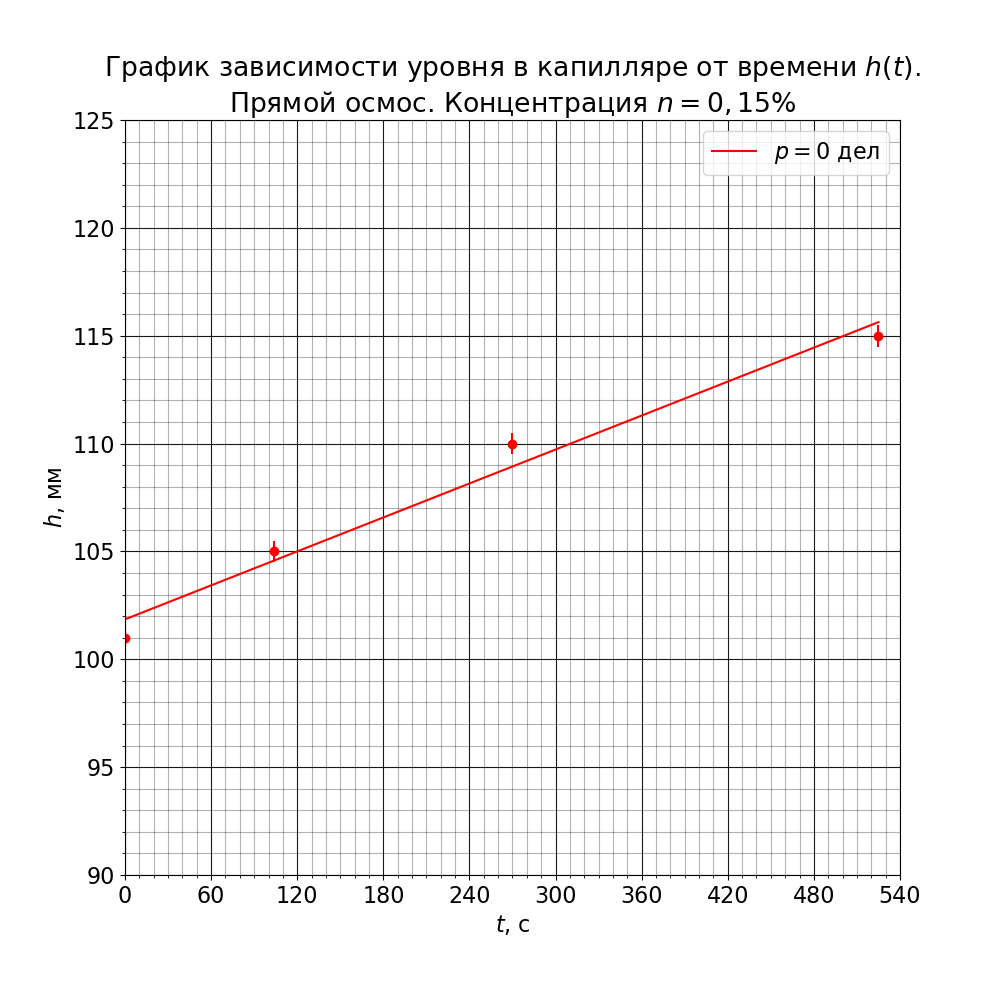
\includegraphics[width=1 \textwidth]{../plots/graph h_t n0.15 straight.png}
\end{figure}

С помощью метода наименьших квадратов проведём наилучшую прямую $h~=~vt~+~h_0$.

$P = 0$ дел. \\
$v = 0,026 \pm 0,003$ $\frac{мм}{с}$. \\
$h_0 = 101,9 \pm 0,8$ мм.

\begin{figure}[H]
	\centering
	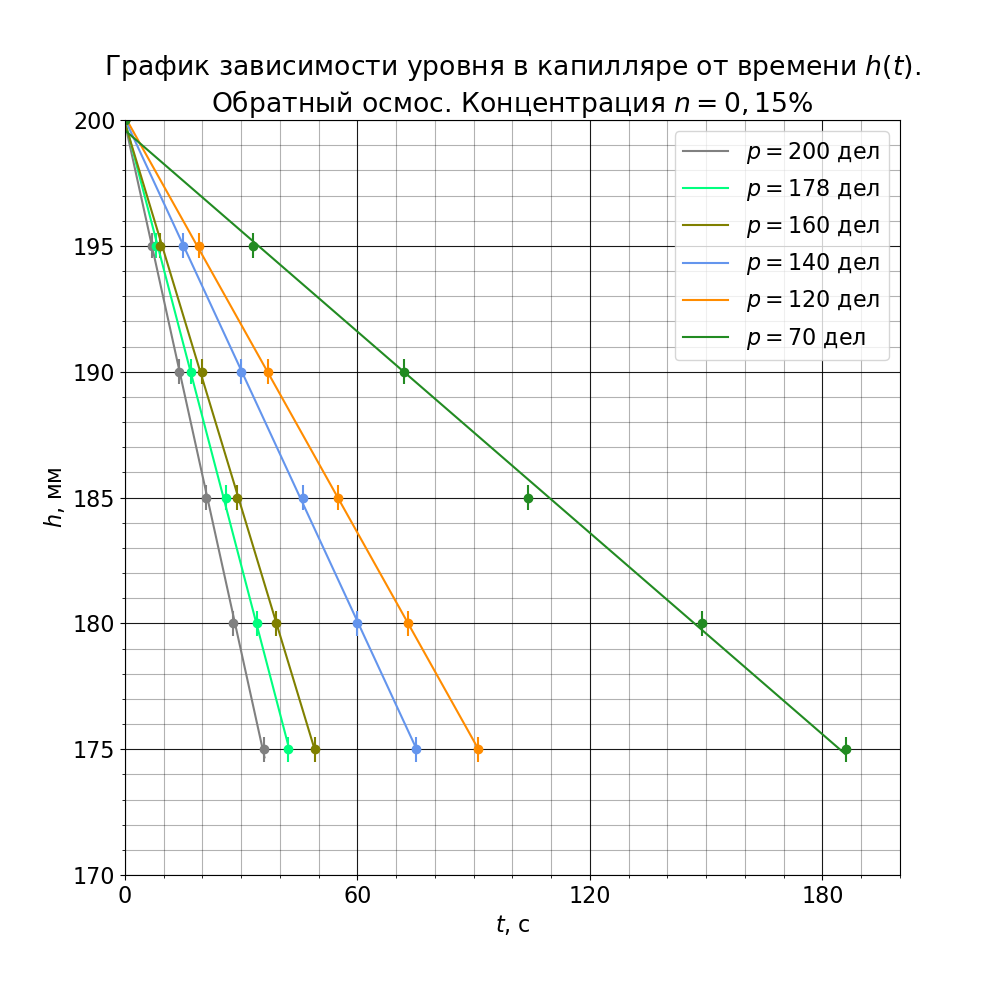
\includegraphics[width=1 \textwidth]{../plots/graph h_t n0.15 reverse.png}
\end{figure}

С помощью метода наименьших квадратов проведём наилучшую прямую $h~=~vt~+~h_0$.

\begin{tabular}[t]{|c|c|c|c|c|c|c|}
\hline
$P$, дел & 200 & 178 & 160 & 140 & 120 & 70 \\ 
\hline
$v$, $\frac{мм}{с}$ & -0,70 & -0,59 & -0,51 & -0,33 & -0,28 & -0,13 \\ 
\hline
$\sigma_v$, $\frac{мм}{с}$ & 0,01 & 0,01 & 0,01 & 0,01 & 0,01 & 0,01 \\ 
\hline
$h_0$, мм & 199,9 & 200,0 & 199,9 & 200,0 & 200,1 & 199,6 \\ 
\hline
$\sigma_{h_0}$, мм & 0,2 & 0,2 & 0,2 & 0,1 & 0,1 & 0,3 \\ 
\hline
\end{tabular}

% n = 0,075%

\begin{figure}[H]
	\centering
	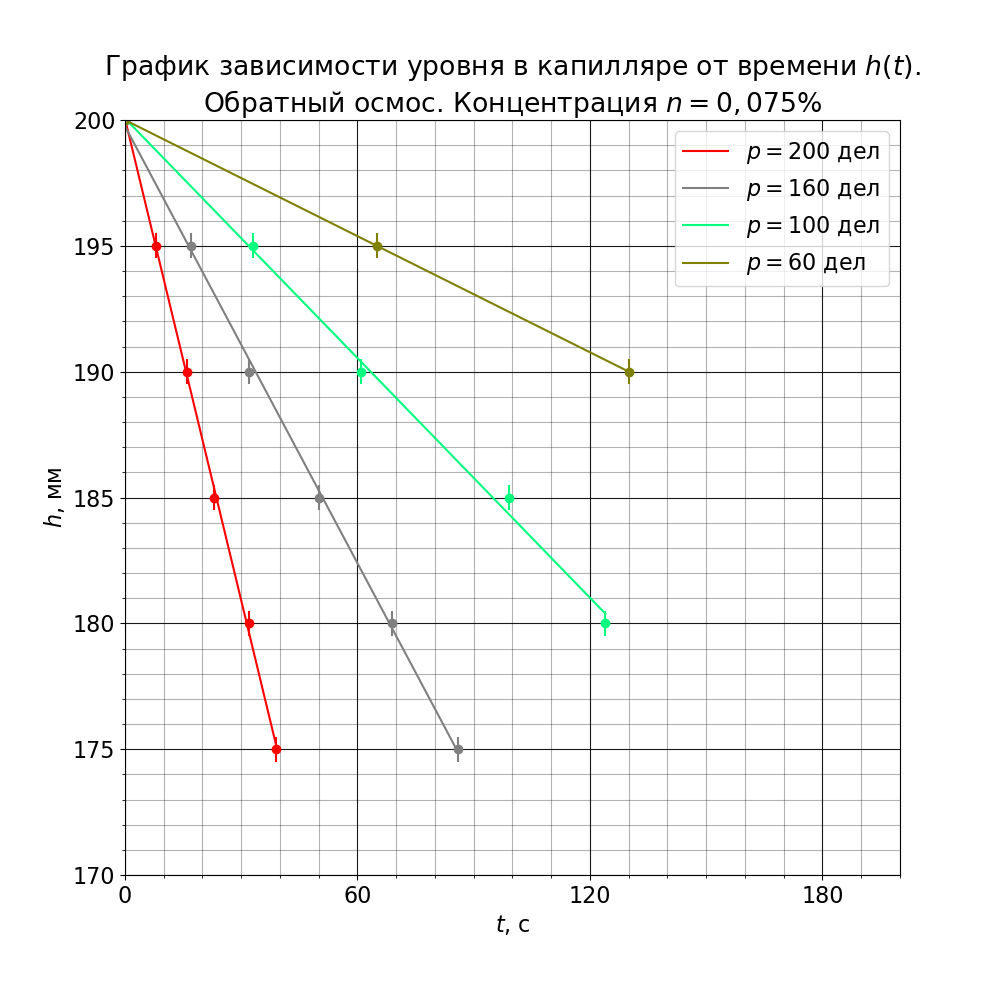
\includegraphics[width=1 \textwidth]{../plots/graph h_t n0.075 reverse.png}
\end{figure}

С помощью метода наименьших квадратов проведём наилучшую прямую $h~=~vt~+~h_0$.

\begin{tabular}[t]{|c|c|c|c|c|}
\hline
$P$, дел & 200 & 160 & 100 & 60 \\
\hline
$v$, $\frac{мм}{с}$ & -0,64 & -0,29 & -0,16 & -0,08 \\
\hline
$\sigma_v$, $\frac{мм}{с}$ & 0,01 & 0,01 & 0,01 & 0,01 \\
\hline
$h_0$, мм & 200,1 & 199,8 & 200,1 & 200,0 \\
\hline
$\sigma_{h_0}$, мм & 0,2 & 0,2 & 0,4 & 0,1 \\
\hline
\end{tabular}

% v(P)

\begin{figure}[H]
	\centering
	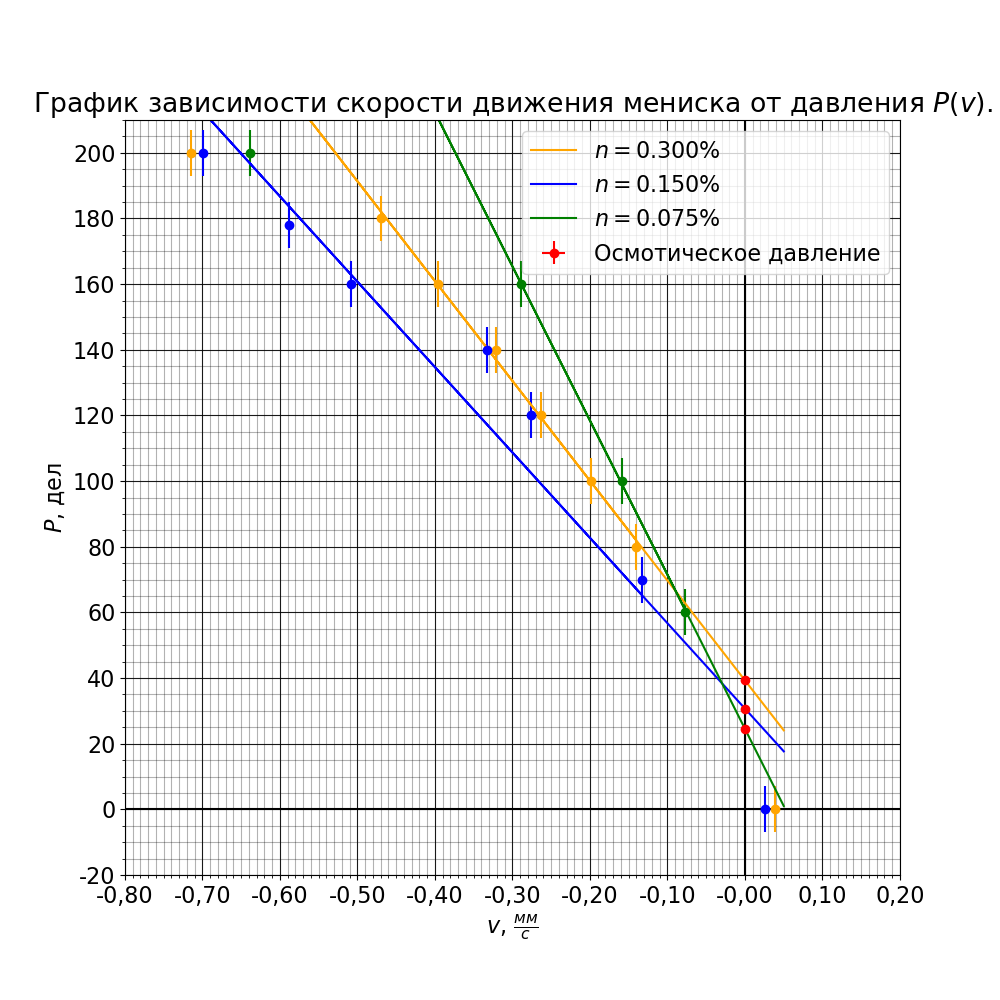
\includegraphics[width = 0.9 \textwidth]{../plots/graph_p_v.png}
\end{figure}

Построим график зависимости давления от скорости, а не скорости от давления, потому что погрешность определения скорости мала, а давление в системе значительно изменялось из-за наличия течи. Тогда можно применить метод наименьших квадратов для проведения прямой $P = av + P_{осм}$.

\begin{tabular}[t]{|c|c|c|c|c|}
\hline
$n$, $\%$ & $a$, $\frac{дел \cdot с}{мм}$ & $\sigma_a$, $\frac{дел \cdot с}{мм}$ & $P_{осм}$, дел & $\sigma_{P_{осм}}$, дел \\ 
\hline
0,300 & -304 & 8 & 39,3 & 2,5 \\ 
0,150 & -260 & 29 & 30,7 & 12,3 \\ 
0,075 & -470 & 8 & 24,5 & 1,6 \\ 
\hline
\end{tabular}

\newpage

По графику видно, что при давлении $P = 200$ делений, экспериментальные точки сильно отклоняются от прямой. Это может быть связано с тем, что при таком давлении существенно влияние течи, которое оказывает сильное воздействие на скорость движения уровня жидкости в капилляре.

Также из общей зависимости отклоняются точки при $P = 0$ делений. Это возможно из-за того, что полупроницаемые перегородки на установке менялись давно, и осмос протекает медленнее.

\newpage

\begin{figure}[H]
	\centering
	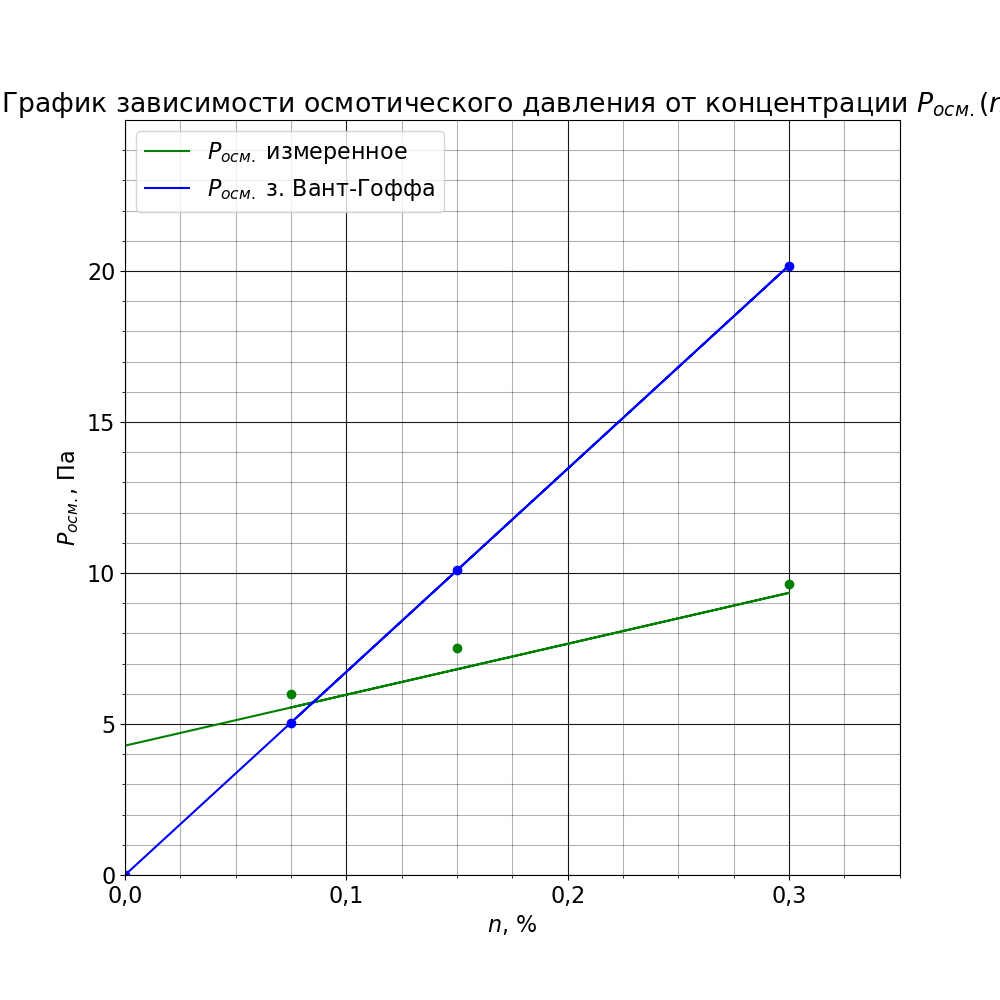
\includegraphics[width=1 \textwidth]{../plots/graph_p_osm_n.png}
\end{figure}

Методом наименьших квадратов по измеренных точкам проведём наилучшую прямую $P~=~an~+~b$. Также построим график зависимости осмотического давления от концентрации по закону Вант-Гоффа.

Коэффициенты МНК. \\
\begin{tabular}[t]{|c|c|c|c|}
\hline
$a$, $10^3$ $\frac{Па}{\%}$ & $\sigma_a$, $10^3$ $\frac{Па}{\%}$ & $b$, $10^3$ Па & $\sigma_b$, $10^3$ Па \\ 
\hline
16,8 & 5,2 & 4,3 & 1,0 \\ 
\hline
\end{tabular}

